
\chapter{Phân tích \& Thiết kế hệ thống}

Chương này trình bày chi tiết về thiết kế kiến trúc hệ thống, bao gồm thiết kể cơ sở dữ liệu (Database), kiến trúc tổng thể, luồng xử lý request, tích hợp AI, thiết kế giao diện người dùng, và kiến trúc mô phỏng 3D. Tất cả các sơ đồ được cung cấp kèm mã PlantUML để dễ dàng chỉnh sửa và tái sử dụng.

\section{Thiết kế Database}

\subsection{Thiết kế Logical Data Model - ERD}

\begin{figure}[H]
    \centering
    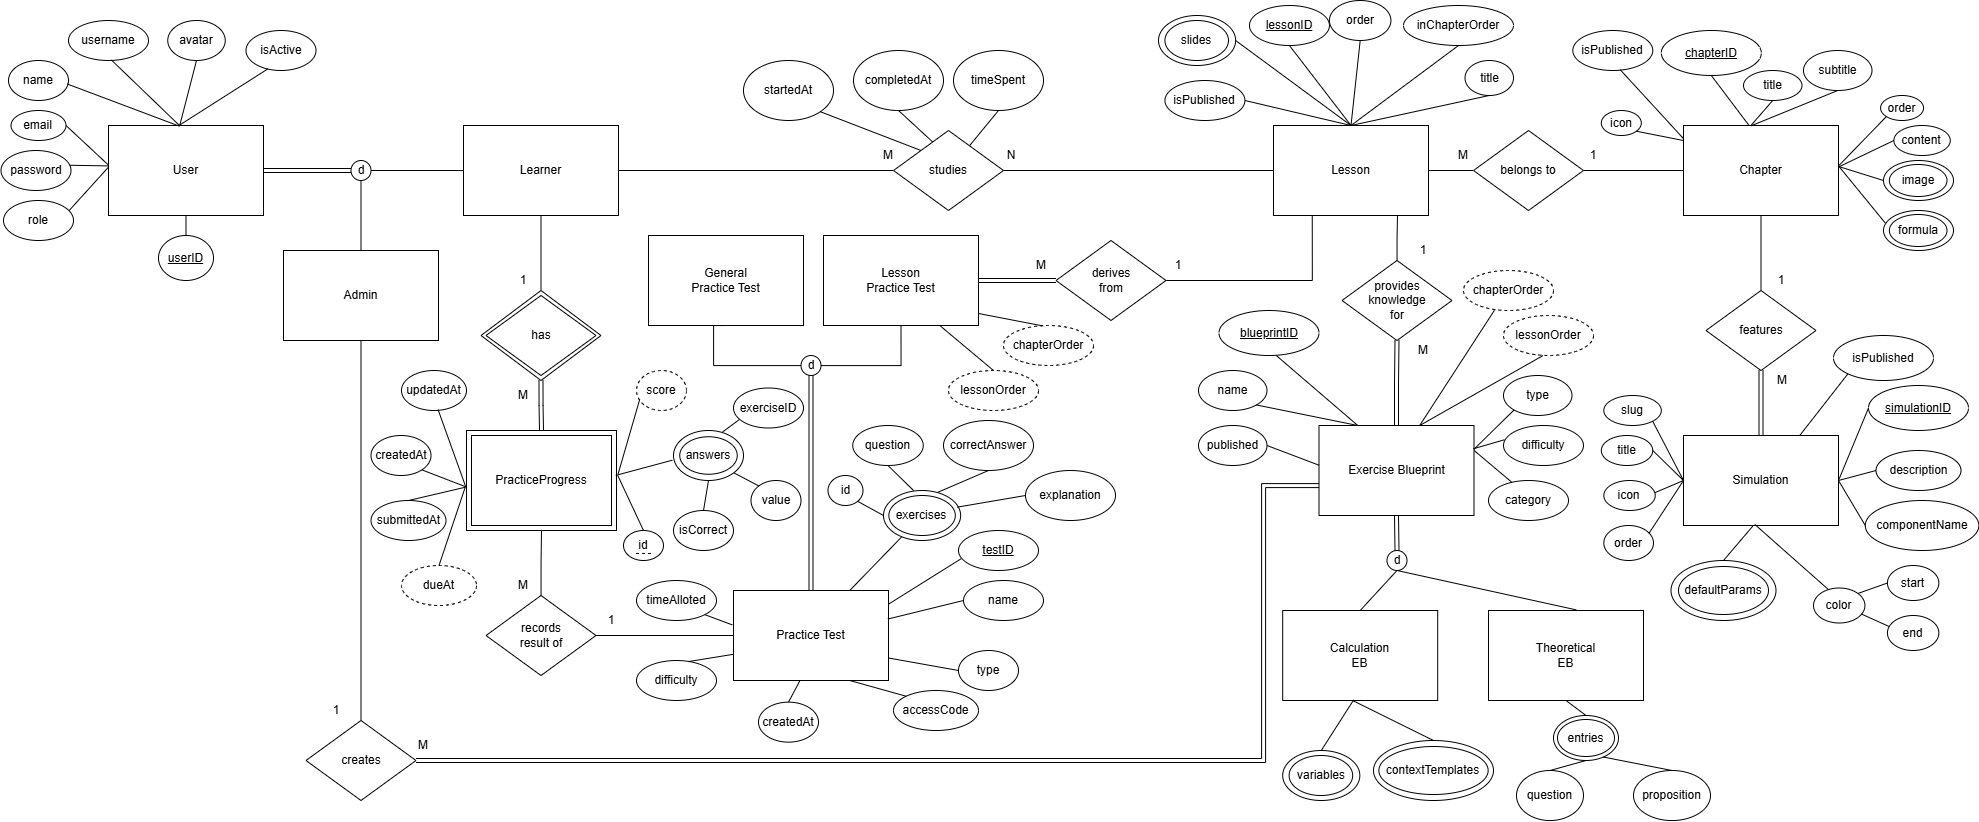
\includegraphics[width=0.95\textwidth]{Images/Phan_tich_Thiet_ke_he_thon/erd.png}
    \vspace{0.5cm}
    \caption{Thiết kế ERD của hệ thống}
    \label{fig:erd} 
\end{figure}

\textbf{Mô tả các kiểu thực thể (Entity Types)}

\begin{itemize}

% ================= USER =================
\item \textbf{Entity type \texttt{User} (Người dùng)}:
\begin{itemize}
    \item \textbf{Mô tả}: Đại diện cho toàn bộ người dùng trong hệ thống, bao gồm người học và quản trị viên.
    
    \item \textbf{Các thuộc tính}:
    \begin{itemize}
        \item \texttt{userID}: khóa chính
        \item \texttt{username}: tên đăng nhập
        \item \texttt{name}: họ tên người dùng
        \item \texttt{email}: email đăng nhập
        \item \texttt{password}: mật khảu tài khoản
        \item \texttt{role}: vai trò, gồm 2 giá trị Learner và Admin
        \item \texttt{avatar}: hình đại điện
        \item \texttt{isActive}: trạng thái hoạt động
    \end{itemize}

    \item \textbf{Chuyên biệt hóa}: ràng buộc \textbf{disjoint}.
    \begin{itemize}
        \item Learner
        \item Admin
    \end{itemize}
\end{itemize}


% ================= LEARNER =================
\item \textbf{Entity type \texttt{Learner} (Người học)}:
\begin{itemize}
    \item \textbf{Mô tả}: Người dùng tham gia học tập và làm đề luyện tập.
    \item \textbf{Thuộc tính}: kế thừa từ User, không có thuộc tính riêng.
\end{itemize}


% ================= ADMIN =================
\item \textbf{Entity type \texttt{Admin} (Quản trị viên)}:
\begin{itemize}
    \item \textbf{Mô tả}: Người quản lý nội dung hệ thống.
    \item \textbf{Thuộc tính}: kế thừa từ User, không có thuộc tính riêng.
\end{itemize}


% ================= PRACTICE PROGRESS =================
\item \textbf{Entity type \texttt{PracticeProgress}}:
\begin{itemize}
    \item \textbf{Mô tả}: Ghi nhận tiến trình làm đề luyện tập của người học.
    
    \item \textbf{Các thuộc tính}:
    \begin{itemize}
        \item \texttt{id}: khóa một phần
        \item \texttt{createdAt}: thời điểm khởi tạo
        \item \texttt{updatedAt}: thời điểm cập nhật gần nhất
        \item \texttt{submittedAt}: thời điểm nộp bài
        \item \texttt{dueAt}: thời hạn nộp bài, thuộc tính dẫn xuất
        \item \texttt{score}: điểm cho bài làm, thuộc tính dẫn xuất
        \item \texttt{answers}: chi tiết bài làm, thuộc tính phức hợp gồm \texttt{value} (nội dung câu trả lời) và \texttt{isCorrect} (đúng/sai)
    \end{itemize}
    
    \item \textbf{Loại}: thực thể yếu.
\end{itemize}


% ================= PRACTICE TEST =================
\item \textbf{Entity type \texttt{Practice Test}}:
\begin{itemize}
    \item \textbf{Mô tả}: Đề luyện tập trong hệ thống.
    
    \item \textbf{Các thuộc tính}:
    \begin{itemize}
        \item \texttt{testID}: khóa chính
        \item \texttt{name}: tên hiển thị
        \item \texttt{type}: loại hình đề, gồm 2 giá trị General (Đề tổng hợp) và Lesson (Đề theo bài học)
        \item \texttt{difficulty}: độ khó
        \item \texttt{timeAlloted}: thời gian cho phép làm bài
        \item \texttt{createdAt}: thời điểm khởi tạo
        \item \texttt{accessCode}: code truy cập làm bài
        \item \texttt{exercises}: bài tập trong đề, thuộc tính phức hợp gồm \texttt{question} (câu hỏi), \texttt{correctAnswer} (câu trả lời đúng) và \texttt{explanation} (giải thích kết quả)
    \end{itemize}

    \item \textbf{Chuyên biệt hóa}: ràng buộc \textbf{disjoint}.
    \begin{itemize}
        \item General Practice Test
        \item Lesson Practice Test
    \end{itemize}
\end{itemize}


% ================= LESSON =================
\item \textbf{Entity type \texttt{Lesson}}:
\begin{itemize}
    \item \textbf{Mô tả}: Bài học trong hệ thống.
    
    \item \textbf{Các thuộc tính}:
    \begin{itemize}
        \item \texttt{lessonID}: khóa chính
        \item \texttt{title}: tiêu đề bài học
        \item \texttt{order}: thứ tự hiển thị
        \item \texttt{slides}: slide bài học, thuộc tính đa trị
    \end{itemize}
\end{itemize}


% ================= CHAPTER =================
\item \textbf{Entity type \texttt{Chapter}}:
\begin{itemize}
    \item \textbf{Mô tả}: Chương học chứa nhiều bài học.
    
    \item \textbf{Các thuộc tính}:
    \begin{itemize}
        \item \texttt{chapterID}: khóa chính
        \item \texttt{title}: tiêu đề chương
        \item \texttt{subtitle}: phụ đề chương
        \item \texttt{order}: thứ tự hiển thị
        \item \texttt{content}: tóm tắt nội dung chương
        \item \texttt{image}: hình ảnh trong chương, thuộc tính đa trị
        \item \texttt{formula}: công thức trong chương, thuộc tính đa trị
        \item \texttt{icon}: biểu tượng hiển thị
        \item \texttt{isPublished}: trạng thái xuất bản
    \end{itemize}
\end{itemize}


% ================= EXERCISE BLUEPRINT =================
\item \textbf{Entity type \texttt{Exercise Blueprint}}:
\begin{itemize}
    \item \textbf{Mô tả}: Khung định nghĩa bài tập.
    
    \item \textbf{Các thuộc tính}:
    \begin{itemize}
        \item \texttt{blueprintID}: khóa chính
        \item \texttt{name}: tên blueprint
        \item \texttt{type}: loại hình blueprint, gồm 2 giá trị Multiple-choice (trắc nghiệm) và Numeric-input (Điền số)
        \item \texttt{difficulty}: dộ khó
        \item \texttt{category}: loại hình câu hỏi, gồm các giá trị Calculation (tính toán), Theory (lý thuyết), ...
    \end{itemize}

    \item \textbf{Chuyên biệt hóa (disjointed)}:
    \begin{itemize}
        \item Calculation EB
        \item Theoretical EB
    \end{itemize}
\end{itemize}


% ================= SIMULATION =================
\item \textbf{Entity type \texttt{Simulation}}:
\begin{itemize}
    \item \textbf{Mô tả}: Mô phỏng tương tác trong hệ thống.
    
    \item \textbf{Các thuộc tính}:
    \begin{itemize}
        \item \texttt{simulationID}: khóa chính
        \item \texttt{title}: tiêu đề mô phỏng
        \item \texttt{slug}: đường dẫn thân thiện
        \item \texttt{order}: thứ tự hiển thị
        \item \texttt{description}: mô tả nội dung mô phỏng
        \item \texttt{componentName}: component tương ứng
        \item \texttt{isPublished}: trạng thái xuất bản
        \item \texttt{defaultParams}: tham số mặc định, thuộc tính đa trị
        \item \texttt{color}: màu sắc gradient, thuộc tính kết hợp giữa \texttt{start} và \texttt{end}
        \item \texttt{start}
        \item \texttt{end}
    \end{itemize}
\end{itemize}

% ================= GENERAL PRACTICE TEST =================
\item \textbf{Entity type \texttt{General Practice Test}}:
\begin{itemize}
    \item \textbf{Mô tả}: Bài kiểm tra thực hành tổng quát, không gắn với một bài học cụ thể.
    \item \textbf{Thuộc tính}: kế thừa từ Practice Test, không có thuộc tính riêng.
\end{itemize}


% ================= LESSON PRACTICE TEST =================
\item \textbf{Entity type \texttt{Lesson Practice Test}}:
\begin{itemize}
    \item \textbf{Mô tả}: Bài kiểm tra thực hành được sinh ra từ một bài học cụ thể.
    \item \textbf{Thuộc tính}: kế thừa từ Practice Test.
    \item \textbf{Thuộc tính mở rộng}:
    \begin{itemize}
        \item lesson order: thứ tự bài học
        \item chapter order: thứ tự chương
    \end{itemize}
\end{itemize}


% ================= CALCULATION EB =================
\item \textbf{Entity type \texttt{Calculation EB}}:
\begin{itemize}
    \item \textbf{Mô tả}: Loại Exercise Blueprint dành cho các bài toán tính toán.
    
    \item \textbf{Thuộc tính}: kế thừa từ Exercise Blueprint.
    
    \item \textbf{Thuộc tính mở rộng}:
    \begin{itemize}
        \item variables: các biến đầu vào, thuộc tính đa trị
        \item equations: các phương trình, thuộc tính đa trị
    \end{itemize}
\end{itemize}


% ================= MULTIPLE CHOICE EB =================
\item \textbf{Entity type \texttt{Multiple-choice EB}}:
\begin{itemize}
    \item \textbf{Mô tả}: Loại Exercise Blueprint dạng trắc nghiệm.
    
    \item \textbf{Thuộc tính}: kế thừa từ Exercise Blueprint.
    
    \item \textbf{Thuộc tính mở rộng}:
    \begin{itemize}
        \item optionTemplates: tập lựa chọn đáp án, thuộc tính đa trị
        \item correctAnswerTemplate: đáp án đúng
    \end{itemize}
\end{itemize}

\end{itemize}

\textbf{Các mối liên kết (Relationships)}

\begin{itemize}

% ================= STUDIES =================
\item \textbf{Relationship \texttt{Studies}}:
\begin{itemize}
    \item \textbf{Giữa}: Learner và Lesson
    \item \textbf{Loại quan hệ}: nhiều - nhiều (M-N)
    \item \textbf{Thuộc tính}:
    \begin{itemize}
        \item \texttt{startedAt}: thời gian bắt đầu học
        \item \texttt{completedAt}: thời gian hoàn thành
        \item \texttt{timeSpent}: thời gian học
    \end{itemize}
    \item \textbf{Mô tả}: Ghi nhận quá trình học của người học đối với từng bài học.
\end{itemize}


% ================= HAS =================
\item \textbf{Relationship \texttt{Has} (Identifying Relationship)}:
\begin{itemize}
    \item \textbf{Giữa}: Learner và PracticeProgress
    \item \textbf{Loại quan hệ}: một - nhiều (1-M)
    \item \textbf{Ràng buộc}: tham gia toàn phần với PracticeProgress
    \item \textbf{Mô tả}: Mỗi tiến trình làm bài thuộc về đúng một người học.
\end{itemize}


% ================= RECORDS RESULT OF =================
\item \textbf{Relationship \texttt{Records result of}}:
\begin{itemize}
    \item \textbf{Giữa}: PracticeProgress và Practice Test
    \item \textbf{Loại quan hệ}: nhiều - một (M-1)
    \item \textbf{Mô tả}: Ghi nhận kết quả làm bài của một lần thực hiện bài kiểm tra.
\end{itemize}


% ================= CREATES =================
\item \textbf{Relationship \texttt{Creates}}:
\begin{itemize}
    \item \textbf{Giữa}: Admin và Practice Test
    \item \textbf{Loại quan hệ}: một - nhiều (1-M)
    \item \textbf{Mô tả}: Quản trị viên tạo ra các bài kiểm tra trong hệ thống.
\end{itemize}


% ================= DERIVES FROM =================
\item \textbf{Relationship \texttt{Derives from}}:
\begin{itemize}
    \item \textbf{Giữa}: Lesson Practice Test và Lesson
    \item \textbf{Loại quan hệ}: nhiều - một (M-1)
    \item \textbf{Mô tả}: Bài kiểm tra được sinh ra từ một bài học cụ thể.
\end{itemize}


% ================= BELONGS TO =================
\item \textbf{Relationship \texttt{Belongs to}}:
\begin{itemize}
    \item \textbf{Giữa}: Lesson và Chapter
    \item \textbf{Loại quan hệ}: nhiều - một (M-1)
    \item \textbf{Mô tả}: Mỗi bài học thuộc về một chương học.
\end{itemize}


% ================= PROVIDES KNOWLEDGE FOR =================
\item \textbf{Relationship \texttt{Provides knowledge for}}:
\begin{itemize}
    \item \textbf{Giữa}: Lesson và Exercise Blueprint
    \item \textbf{Loại quan hệ}: một - nhiều (1-M)
    \item \textbf{Mô tả}: Bài học cung cấp kiến thức cho các khung bài tập tương ứng.
\end{itemize}


% ================= FEATURES =================
\item \textbf{Relationship \texttt{Features}}:
\begin{itemize}
    \item \textbf{Giữa}: Chapter và Simulation
    \item \textbf{Loại quan hệ}: một - nhiều (1-M)
    \item \textbf{Mô tả}: Mỗi chương có thể chứa nhiều mô phỏng tương tác.
\end{itemize}

\end{itemize}


\subsection{Thiết kế Physical Data Model - Document Schema}

Hệ thống sử dụng \textbf{MongoDB} làm cơ sở dữ liệu, với mô hình dữ liệu dạng \textbf{document-based} (NoSQL). Hệ thống bao gồm các collection (màu xanh) và embedded document (màu đỏ) như trong hình dưới.

\begin{figure}[H]
    \centering
    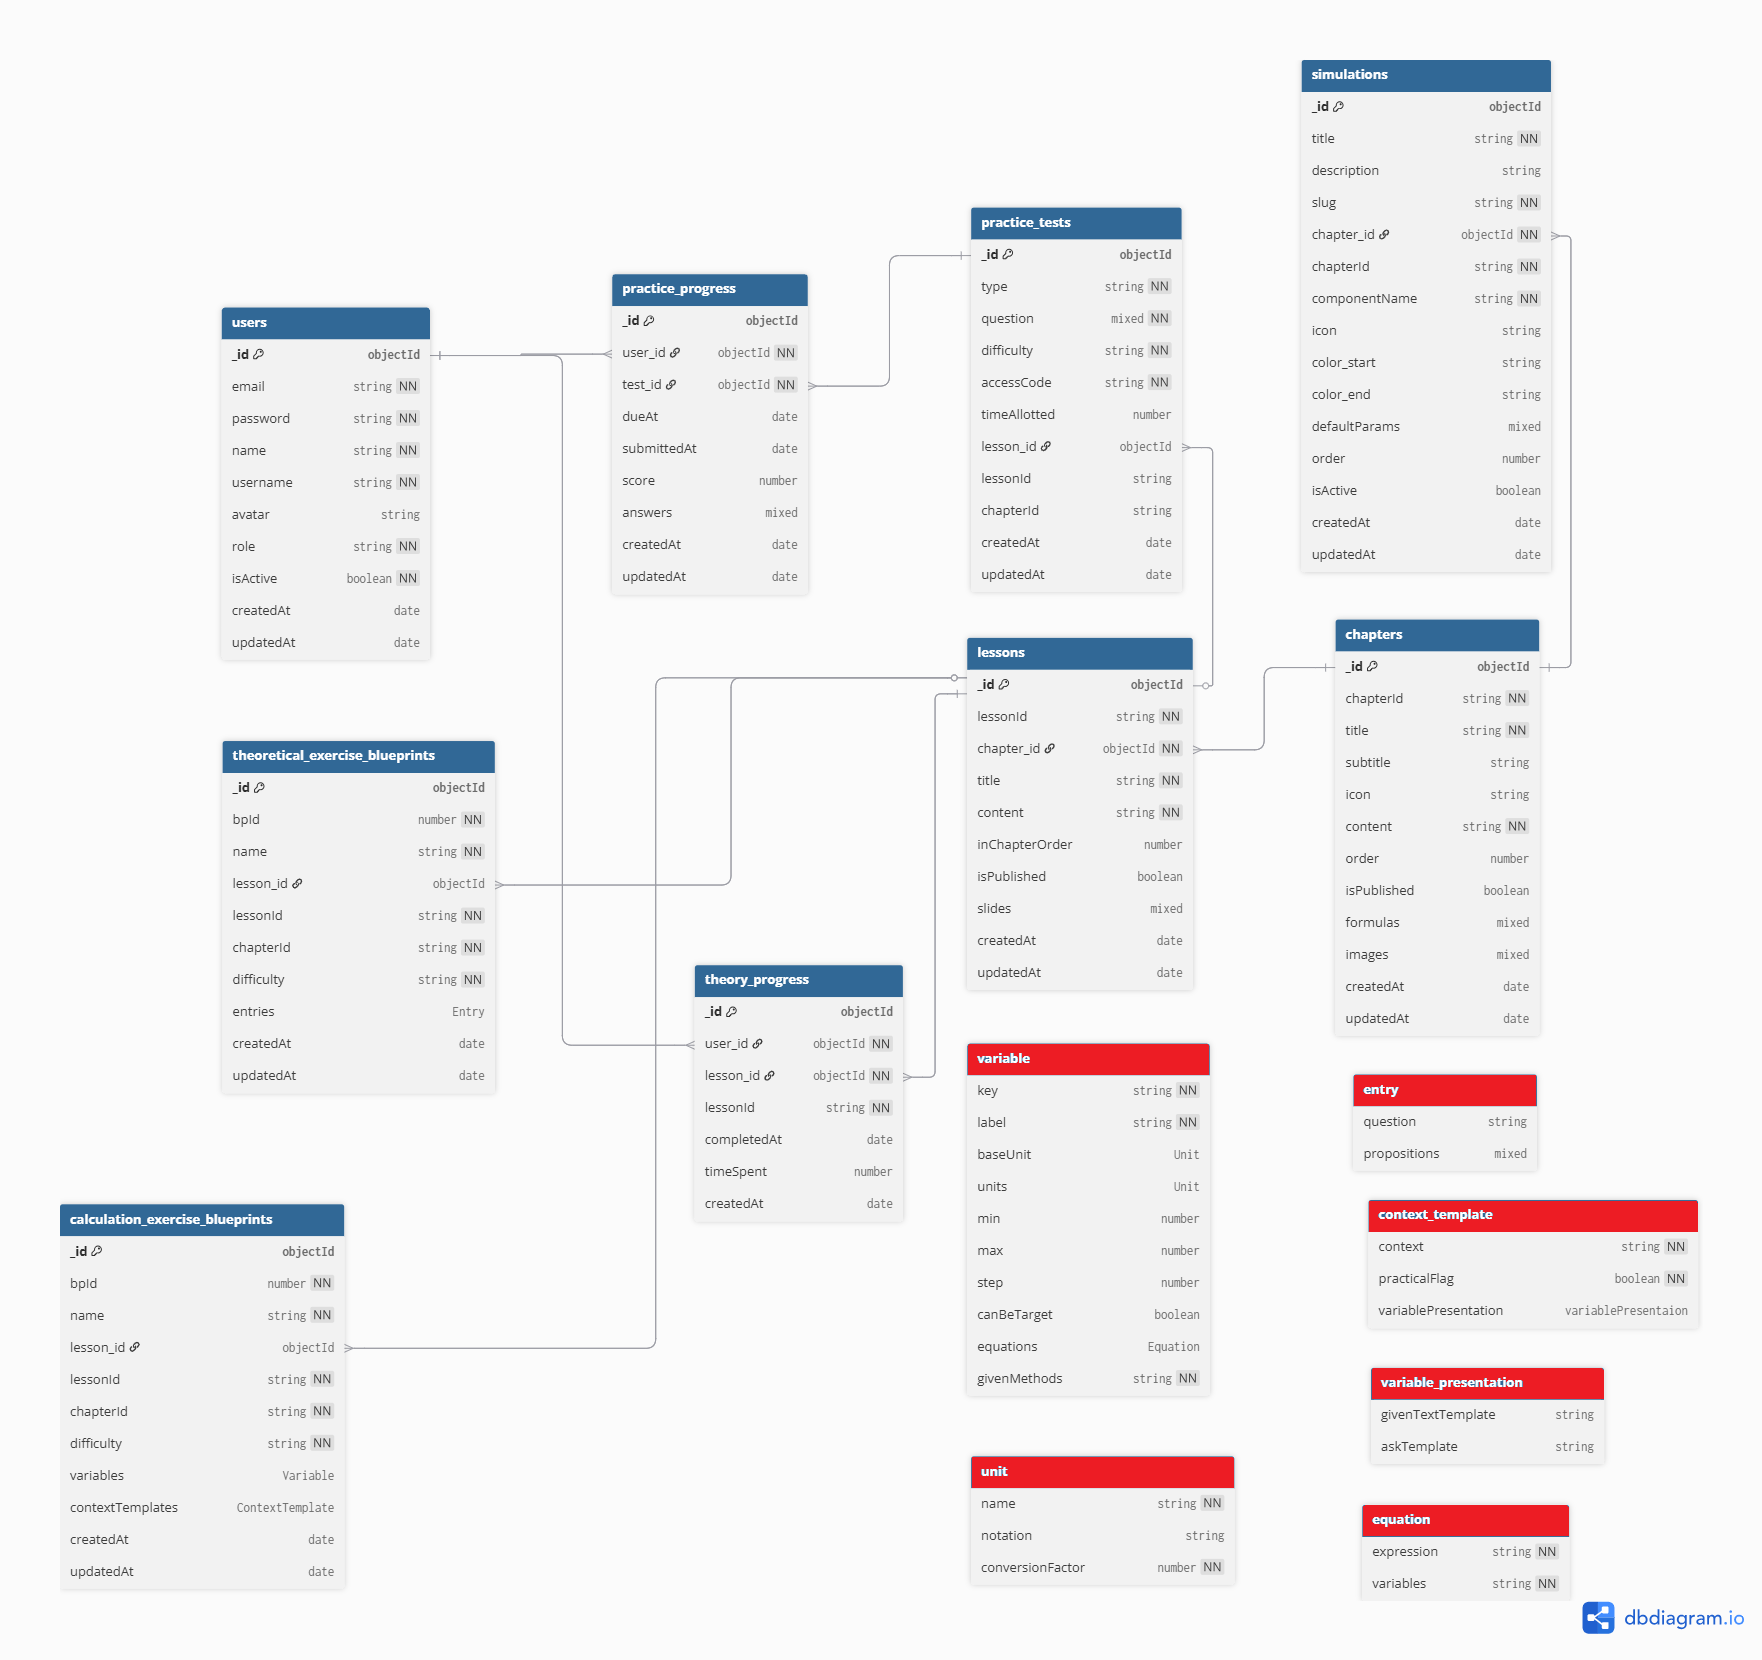
\includegraphics[width=0.75\textwidth]{Images/Phan_tich_Thiet_ke_he_thon/Document-Schema.png}
    \vspace{0.5cm}
    \caption{Thiết kế Document Schema của hệ thống}
    \label{fig:erd}
\end{figure}

\begin{enumerate}
    \item \textbf{Collection \texttt{users} (Người dùng)}:
    \begin{itemize}
        \item \textbf{Mục đích}: Lưu trữ thông tin tài khoản người dùng trong hệ thống học tập (học sinh, giáo viên, quản trị viên).
        
        \item \textbf{Các trường chính}:
        \begin{itemize}
            \item \texttt{\_id}: ObjectId – khóa chính, tự động sinh bởi MongoDB.
            
            \item \texttt{email}: string – email đăng nhập (duy nhất, unique).
            
            \item \texttt{password}: string – mật khẩu đã mã hóa bằng bcrypt (salt rounds = 10 hoặc 12).
            
            \item \texttt{name}: string – họ tên người dùng.
            
            \item \texttt{username}: string – tên người dùng hiển thị / định danh phụ (unique, bắt buộc).
            
            \item \texttt{avatar}: string | null – URL ảnh đại diện (có thể null).
            
            \item \texttt{role}: "learner" | "admin" – vai trò người dùng trong hệ thống (mặc định: "learner").
            
            \item \texttt{isActive}: boolean – trạng thái kích hoạt tài khoản (mặc định: true).
            
            \item \texttt{createdAt}, \texttt{updatedAt}: Date – thời gian tạo và cập nhật tự động.
        \end{itemize}
        
        \item \textbf{Dữ liệu mẫu}:
        \begin{verbatim}
        {
          "email": "admin@physicsbook.com",
          "password": "$2b$10$...",
          "name": "Administrator",
          "username": "admin",
          "role": "admin",
          "isActive": true
        }
        \end{verbatim}
    \end{itemize}

    \item \textbf{Collection \texttt{chapters} (Chương học)}:
    \begin{itemize}
        \item \textbf{Mục đích}: Lưu trữ nội dung các chương học trong hệ thống học tập.
    
        \item \textbf{Các trường chính}:
        \begin{itemize}
            \item \texttt{\_id}: ObjectId – khóa chính, tự động sinh bởi MongoDB.
            
            \item \texttt{chapterId}: string – mã định danh chương học (unique, ví dụ: "chapter-1").
            
            \item \texttt{title}: string – tiêu đề chương học.
            
            \item \texttt{subtitle}: string – phụ đề chương học.
            
            \item \texttt{icon}: string – đường dẫn hoặc tên icon đại diện chương.
            
            \item \texttt{content}: string – nội dung mô tả chính của chương.
            
            \item \texttt{order}: number – thứ tự hiển thị chương (mặc định: 0).
            
            \item \texttt{isPublished}: boolean – trạng thái xuất bản (mặc định: true).
            
            \item \texttt{formulas}: mixed – danh sách công thức liên quan (dữ liệu linh hoạt).
            
            \item \texttt{images}: mixed – danh sách hình ảnh minh hoạ (dữ liệu linh hoạt).
            
            \item \texttt{createdAt}, \texttt{updatedAt}: Date – thời gian tạo và cập nhật tự động.
        \end{itemize}
    
        \item \textbf{Dữ liệu mẫu}:
        \begin{verbatim}
        {
          "chapterId": "chapter-1",
          "title": "Chương 1: Dao Động",
          "subtitle": "Dao động cơ bản và điều hòa",
          "icon": "oscillation-icon.png",
          "content": "Giới thiệu về dao động cơ học...",
          "order": 1,
          "isPublished": true,
          "formulas": [],
          "images": []
        }
        \end{verbatim}
    
    \end{itemize}

    \item \textbf{Collection \texttt{Lesson} (Bài học)}:
        \begin{itemize}
            \item \textbf{Mục đích}: Lưu trữ nội dung bài học thuộc về một chương (\texttt{Chapter}), bao gồm nội dung văn bản và các slides đi kèm.
        
            \item \textbf{Các trường chính}:
            \begin{itemize}
                \item \texttt{\_id}: ObjectId – khóa chính của MongoDB.
                \item \texttt{lessonId}: string – mã bài học (e.g., "1", "2").
                \item \texttt{chapter\_id}: ObjectId – tham chiếu đến chương chứa bài học (\texttt{chapters.\_id}).
                \item \texttt{title}: string – tiêu đề bài học.
                \item \texttt{content}: string – nội dung chính của bài học.
                \item \texttt{slides}: Mixed – danh sách slides (cấu trúc linh hoạt, embedded documents).
                \item \texttt{inChapterOrder}: number – thứ tự bài học trong chương.
                \item \texttt{isPublished}: boolean – trạng thái hiển thị bài học (mặc định: true).
                \item \texttt{createdAt}: date – thời gian tạo.
                \item \texttt{updatedAt}: date – thời gian cập nhật gần nhất.
            \end{itemize}
        
            \item \textbf{Dữ liệu mẫu}:
            \begin{verbatim}
            {
              "_id": "64f1c2a9...",
              "lessonId": "1",
              "chapter_id": "64e9a1b2...",
              "title": "Mô tả dao động",
              "content": "Dao động là ...",
              "slides": [
                ...
              ],
              "inChapterOrder": 1,
              "isPublished": true,
              "createdAt": "2026-05-11",
              "updatedAt": "2026-05-11"
            }
            \end{verbatim}
        \end{itemize}

    \item \textbf{Embedded Document \texttt{Slide} (Slide trình chiếu)}:
    \begin{itemize}
        \item \textbf{Cấu trúc}: Mỗi slide là một document nhúng trong mảng \texttt{slides} của lesson.
        \item \textbf{Các trường chính}:
        \begin{itemize}
            \item \texttt{id}: number – số thứ tự slide.
            \item \texttt{title}: string – tiêu đề slide.
            \item \texttt{type}: string – loại slide: "intro", "foundation", "example", "exploratory", "summary".
            \item \texttt{subId}: number? – sub-id để nhóm các slide cùng chủ đề.
            \item \texttt{content}: string – nội dung HTML của slide (có chứa class Tailwind CSS).
        \end{itemize}
        \item \textbf{Đặc điểm}: Nội dung slide sử dụng HTML với các class Tailwind CSS để định dạng, và MathJax/KaTeX để hiển thị công thức toán học.
    \end{itemize}

    \item \textbf{Collection \texttt{exerciseblueprints} (Blueprint bài tập)}:
    \begin{itemize}
        \item \textbf{Mục đích}: Lưu trữ các mẫu bài tập (template) phục vụ cơ chế sinh đề động dựa trên biến số và context.
    
        \item \textbf{Các trường chính}:
        \begin{itemize}
            \item \texttt{\_id}: ObjectId – khóa chính.
    
            \item \texttt{bpId}: number – mã blueprint.
    
            \item \texttt{name}: string – tên blueprint.
    
            \item \texttt{lesson\_id}: ObjectId | null – tham chiếu bài học.
    
            \item \texttt{lessonId}: string – mã bài học logic.
    
            \item \texttt{chapterId}: string – mã chương học.
    
            \item \texttt{difficulty}: string – "basic" | "intermediate" | "advanced".
    
            \item \texttt{entries}: Entry[] – danh sách câu hỏi (embedded document).
    
            \item \texttt{variables}: Variable – cấu hình biến (embedded document).
    
            \item \texttt{contextTemplates}: ContextTemplate – danh sách context (embedded document).
    
            \item \texttt{createdAt}, \texttt{updatedAt}: Date – thời gian tạo và cập nhật.
        \end{itemize}
    \end{itemize}
    
    % ==========================
    % PRACTICE TESTS
    % ==========================
    
    \item \textbf{Collection \texttt{practice\_tests} (Bài kiểm tra)}:
    \begin{itemize}
        \item \textbf{Mục đích}: Lưu trữ bài kiểm tra trắc nghiệm và tự luận.
    
        \item \textbf{Các trường chính}:
        \begin{itemize}
            \item \texttt{\_id}: ObjectId.
    
            \item \texttt{type}: string – "general" | "lesson" (discriminator).
    
            \item \texttt{question}: mixed – nội dung câu hỏi.
    
            \item \texttt{difficulty}: string – mức độ.
    
            \item \texttt{accessCode}: string – mã truy cập.
    
            \item \texttt{timeAllotted}: number – thời gian làm bài.
    
            \item \texttt{lesson\_id}: ObjectId | null.
    
            \item \texttt{lessonId}: string.
    
            \item \texttt{chapterId}: string.
    
            \item \texttt{createdAt}, \texttt{updatedAt}: Date.
        \end{itemize}
    \end{itemize}
    
    % ==========================
    % PRACTICE PROGRESS
    % ==========================
    
    \item \textbf{Collection \texttt{practice\_progresses} (Tiến độ luyện tập)}:
    \begin{itemize}
        \item \textbf{Mục đích}: Theo dõi kết quả làm bài của người dùng.
    
        \item \textbf{Các trường chính}:
        \begin{itemize}
            \item \texttt{\_id}: ObjectId.
    
            \item \texttt{user\_id}: ObjectId – người dùng.
    
            \item \texttt{test\_id}: ObjectId – bài test.
    
            \item \texttt{dueAt}: Date – hạn làm bài.
    
            \item \texttt{submittedAt}: Date – thời gian nộp.
    
            \item \texttt{score}: number – điểm số.
    
            \item \texttt{answers}: mixed – câu trả lời.
    
            \item \texttt{createdAt}, \texttt{updatedAt}: Date.
        \end{itemize}
    \end{itemize}
    
    % ==========================
    % THEORY PROGRESS
    % ==========================
    
    \item \textbf{Collection \texttt{theory\_progress} (Tiến độ lý thuyết)}:
    \begin{itemize}
        \item \textbf{Mục đích}: Theo dõi tiến độ học lý thuyết của người dùng.
    
        \item \textbf{Các trường chính}:
        \begin{itemize}
            \item \texttt{\_id}: ObjectId.
    
            \item \texttt{user\_id}: ObjectId.
    
            \item \texttt{lesson\_id}: ObjectId.
    
            \item \texttt{lessonId}: string.
    
            \item \texttt{completedAt}: Date, thời điểm hoàn thành
    
            \item \texttt{timeSpent}: number, thời gian đã học
    
            \item \texttt{createdAt}: Date, thời điểm bắt đầu
        \end{itemize}
    \end{itemize}
    
    % ==========================
    % SIMULATIONS
    % ==========================
    \item \textbf{Collection \texttt{simulations} (Mô phỏng)}:
    \begin{itemize}
        \item \textbf{Mục đích}: Lưu trữ metadata của các mô phỏng 3D tương tác.
    
        \item \textbf{Các trường chính}:
        \begin{itemize}
            \item \texttt{\_id}: ObjectId – khóa chính.
    
            \item \texttt{title}: string – tiêu đề mô phỏng (tiếng Việt).
    
            \item \texttt{description}: string – mô tả mô phỏng.
    
            \item \texttt{slug}: string – đường dẫn thân thiện (unique).
    
            \item \texttt{componentName}: string – tên React component tương ứng  
            (ví dụ: \texttt{ElectromagneticWave3D}, \texttt{PendulumSimulation}).
    
            \item \texttt{icon}: string – tên icon (Lucide React).
    
            \item \texttt{color}: object – màu gradient gồm:
            \begin{itemize}
                \item \texttt{start}: string
                \item \texttt{end}: string
            \end{itemize}
    
            \item \texttt{defaultParams}: object – tham số mặc định (JSON).
    
            \item \texttt{order}: number – thứ tự hiển thị.
    
            \item \texttt{isActive}: boolean – trạng thái kích hoạt.
    
            \item \texttt{chapterId}: string – mã chương liên quan.
        \end{itemize}
    
        \item \textbf{Dữ liệu mẫu}:
        \begin{verbatim}
        {
          "title": "Con lắc đơn",
          "slug": "con-lac-don",
          "componentName": "PendulumSimulation",
          "icon": "Circle",
          "color": {
            "start": "from-green-500",
            "end": "to-emerald-500"
          },
          "chapterId": "1"
        }
        \end{verbatim}
    \end{itemize}
    
    % ==========================
    % EMBEDDED: ENTRY
    % ==========================
    
    \item \textbf{Embedded Document \texttt{Entry}}:
    \begin{itemize}
        \item \texttt{question}: string
        \item \texttt{propositions}: mixed
    \end{itemize}
    
    % ==========================
    % EMBEDDED: VARIABLE
    % ==========================
    
    \item \textbf{Embedded Document \texttt{Variable}}:
    \begin{itemize}
        \item \texttt{key}: string
        \item \texttt{label}: string
        \item \texttt{baseUnit}: Unit
        \item \texttt{units}: Unit
        \item \texttt{min}, \texttt{max}, \texttt{step}: number
        \item \texttt{canBeTarget}: boolean
        \item \texttt{givenMethods}: string ("text" | "graph")
        \item \texttt{equations}: Equation[]
    \end{itemize}
    
    % ==========================
    % EMBEDDED: UNIT
    % ==========================
    
    \item \textbf{Embedded Document \texttt{Unit}}:
    \begin{itemize}
        \item \texttt{name}: string
        \item \texttt{notation}: string
        \item \texttt{conversionFactor}: number
    \end{itemize}
    
    % ==========================
    % EMBEDDED: EQUATION
    % ==========================
    
    \item \textbf{Embedded Document \texttt{Equation}}:
    \begin{itemize}
        \item \texttt{expression}: string
        \item \texttt{variables}: string[]
    \end{itemize}
    
    % ==========================
    % EMBEDDED: VARIABLE PRESENTATION
    % ==========================
    
    \item \textbf{Embedded Document \texttt{VariablePresentation}}:
    \begin{itemize}
        \item \texttt{givenTextTemplate}: string[]
        \item \texttt{askTemplate}: string[]
    \end{itemize}
    
    % ==========================
    % EMBEDDED: CONTEXT TEMPLATE
    % ==========================
    
    \item \textbf{Embedded Document \texttt{ContextTemplate}}:
    \begin{itemize}
        \item \texttt{context}: string
        \item \texttt{practicalFlag}: boolean
        \item \texttt{variablePresentation}: map<string, VariablePresentation>
    \end{itemize}
    
    \item \textbf{Embedded \texttt{exercises} (Bài tập)}:
    \begin{itemize}
        \item \textbf{Mục đích}: Lưu trữ các bài tập đã được tạo sẵn (cố định).
        \item \textbf{Các trường chính}:
        \begin{itemize}
            \item \texttt{\_id}: ObjectId – khóa chính.
            \item \texttt{id}: number – mã bài tập.
            \item \texttt{chapterId}: string – mã chương (e.g., "1", "2").
            \item \texttt{lessonId}: string – mã bài học.
            \item \texttt{lessonTitle}: string – tiêu đề bài học.
            \item \texttt{type}: "multiple-choice" | "calculation" – loại bài tập.
            \item \texttt{question}: string – nội dung câu hỏi.
            \item \texttt{options}: string[] – các lựa chọn (cho multiple-choice).
            \item \texttt{correctAnswer}: number | number – đáp án đúng (index hoặc giá trị số).
            \item \texttt{explanation}: string – lời giải thích.
            \item \texttt{difficulty}: "basic" | "intermediate" | "advanced" – độ khó.
            \item \texttt{category}: string – phân loại (e.g., "Dạng 1.1", "Lý thuyết", "Bài tập thực tế").
        \end{itemize}
        \item \textbf{Dữ liệu mẫu}:
        \begin{verbatim}
        {
          "id": 2,
          "lessonId": "1",
          "type": "multiple-choice",
          "question": "Dao động tuần hoàn là dao động mà:",
          "options": ["...", "Trạng thái chuyển động lặp lại như cũ...", "..."],
          "correctAnswer": 1,
          "explanation": "..."
        }
        \end{verbatim}
    \end{itemize}

    \item \textbf{Collection \texttt{verificationcodes} (Mã xác thực)}:
    \begin{itemize}
        \item \textbf{Mục đích}: Lưu trữ mã xác thực email khi đăng ký hoặc quên mật khẩu (hiện tại collection đang trống).
        \item \textbf{Các trường chính}:
        \begin{itemize}
            \item \texttt{\_id}: ObjectId – khóa chính.
            \item \texttt{email}: string – email cần xác thực.
            \item \texttt{code}: string – mã xác thực.
            \item \texttt{expiresAt}: DateTime – thời điểm hết hạn.
            \item \texttt{createdAt}: DateTime.
        \end{itemize}
    \end{itemize}
\end{enumerate}
\section{Kiến trúc hệ thống}

\subsection{Kiến trúc tổng thể (System Architecture)}

Hệ thống được xây dựng theo mô hình \textbf{Full-Stack Web Application} với Next.js 14, kết hợp giữa Server-Side Rendering (SSR) cho nội dung tĩnh và Client-Side Rendering (CSR) cho các mô phỏng 3D tương tác.

\begin{figure}[H]
    \centering
    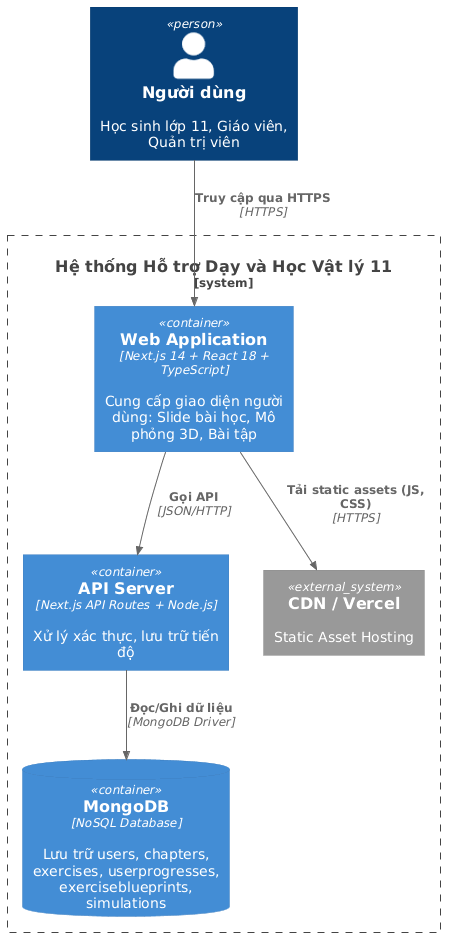
\includegraphics[width=\textwidth,
    height=0.7\textheight,
    keepaspectratio]{Images/Phan_tich_Thiet_ke_he_thon/Architechture.png}
    \vspace{0.5cm}
    \caption{Kiến trúc tổng thể hệ thống}
    \label{fig:system-arch}
\end{figure}


\subsection{Luồng xử lý yêu cầu chính (Request Flow)}

\subsubsection{Luồng 1: Người dùng xem bài học và tương tác với mô phỏng 3D}

\begin{figure}[H]
    \centering
    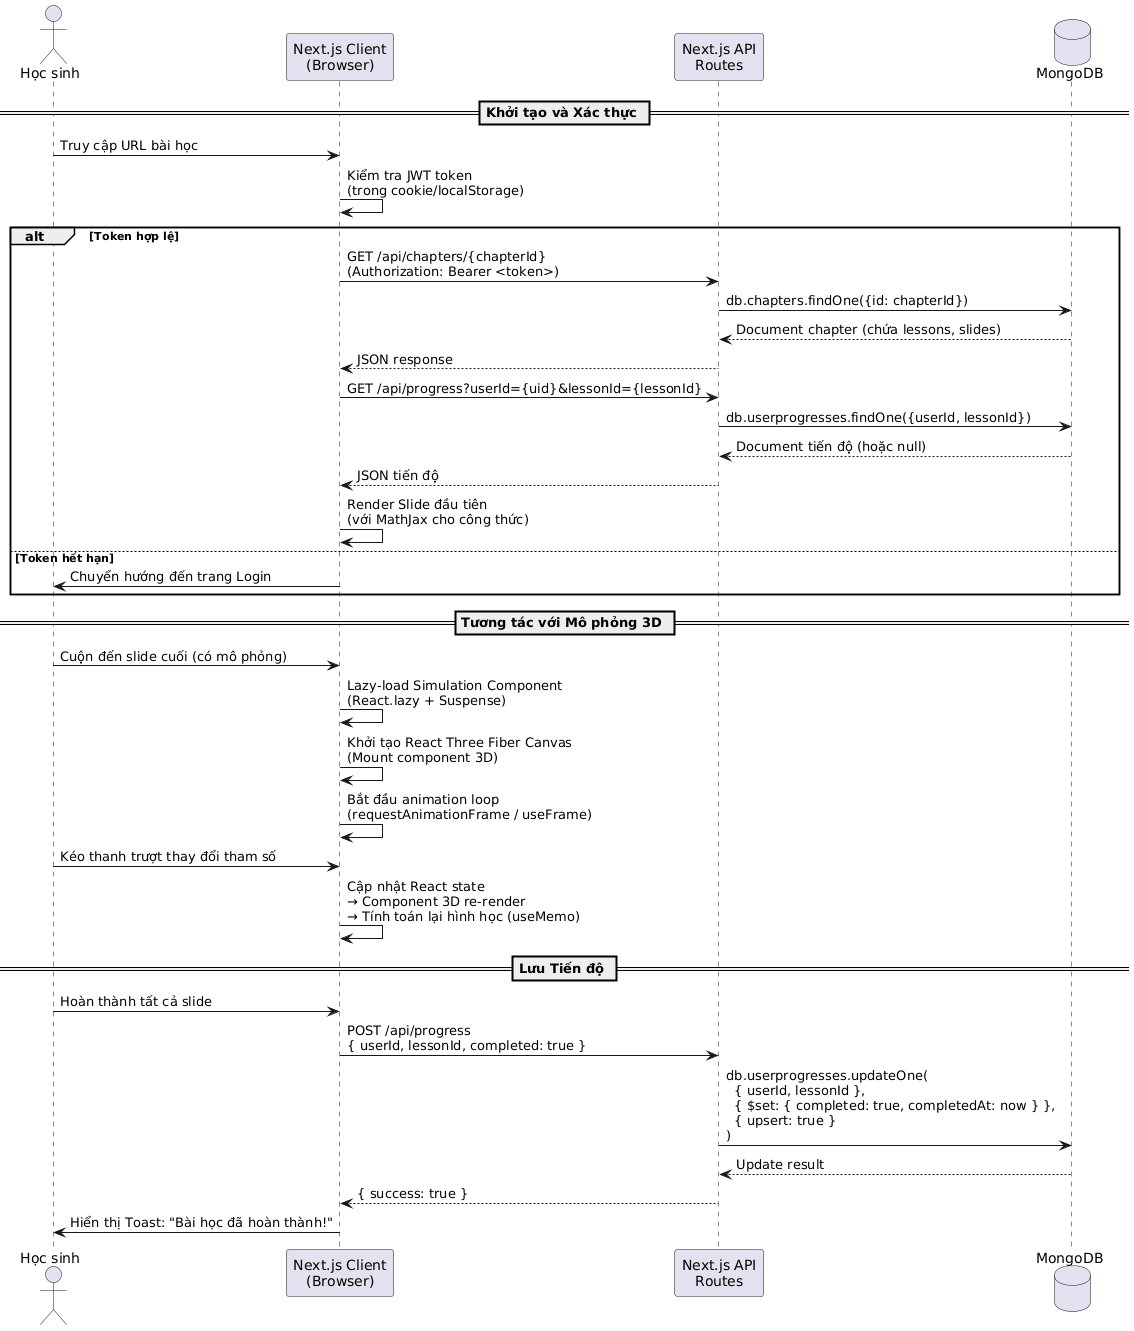
\includegraphics[width=0.75\textwidth]{Images/Phan_tich_Thiet_ke_he_thon/sequence_diagram.png}
    \vspace{0.5cm}
    \caption{Biểu đồ tuần tự: Luồng xem bài học và tương tác với mô phỏng}
    \label{fig:seq-diagram}
\end{figure}


\subsubsection{Luồng 2: Luyện đề và Phân tích}

\begin{figure}[H]
    \centering
    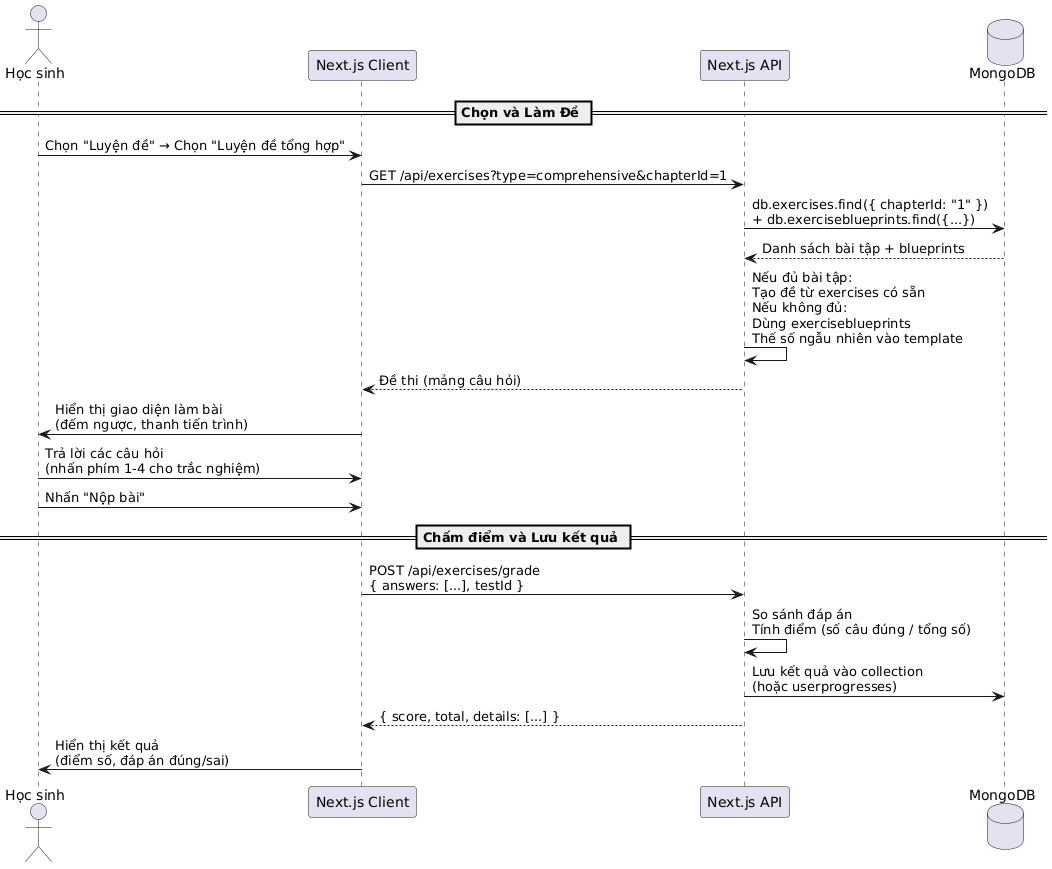
\includegraphics[width=0.65\textwidth]{Images/Phan_tich_Thiet_ke_he_thon/excercise_sequence.png}
    \vspace{0.5cm}
    \caption{Biểu đồ tuần tự: Luồng luyện đề và phân tích kết quả bằng}
    \label{fig:seq-quiz}
\end{figure}

\subsubsection{Luồng 3: Giáo viên tạo phòng, học viên làm bài và xem kết quả}
\begin{figure}[H]
    \centering
    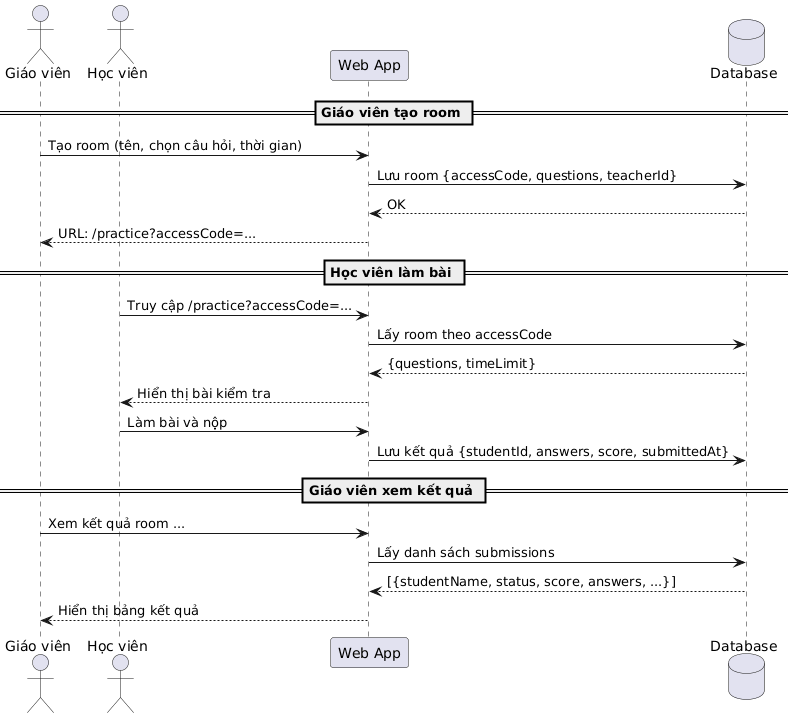
\includegraphics[width=0.65\textwidth]{Images/Phan_tich_Thiet_ke_he_thon/test_room_sequence.png}
    \vspace{0.5cm}
    \caption{Biểu đồ tuần tự: Luồng luyện đề và phân tích kết quả bằng}
    \label{fig:seq-room}
\end{figure}

\section{Thiết kế Kiến trúc Mô phỏng 3D}

\subsection{Kiến trúc Plugin-Based cho Simulation Engine}

Hệ thống mô phỏng 3D được thiết kế theo kiến trúc plugin-based, nơi mỗi mô phỏng là một React component độc lập, có thể được phát triển, kiểm thử và tích hợp riêng biệt.

\begin{figure}[H]
    \centering
    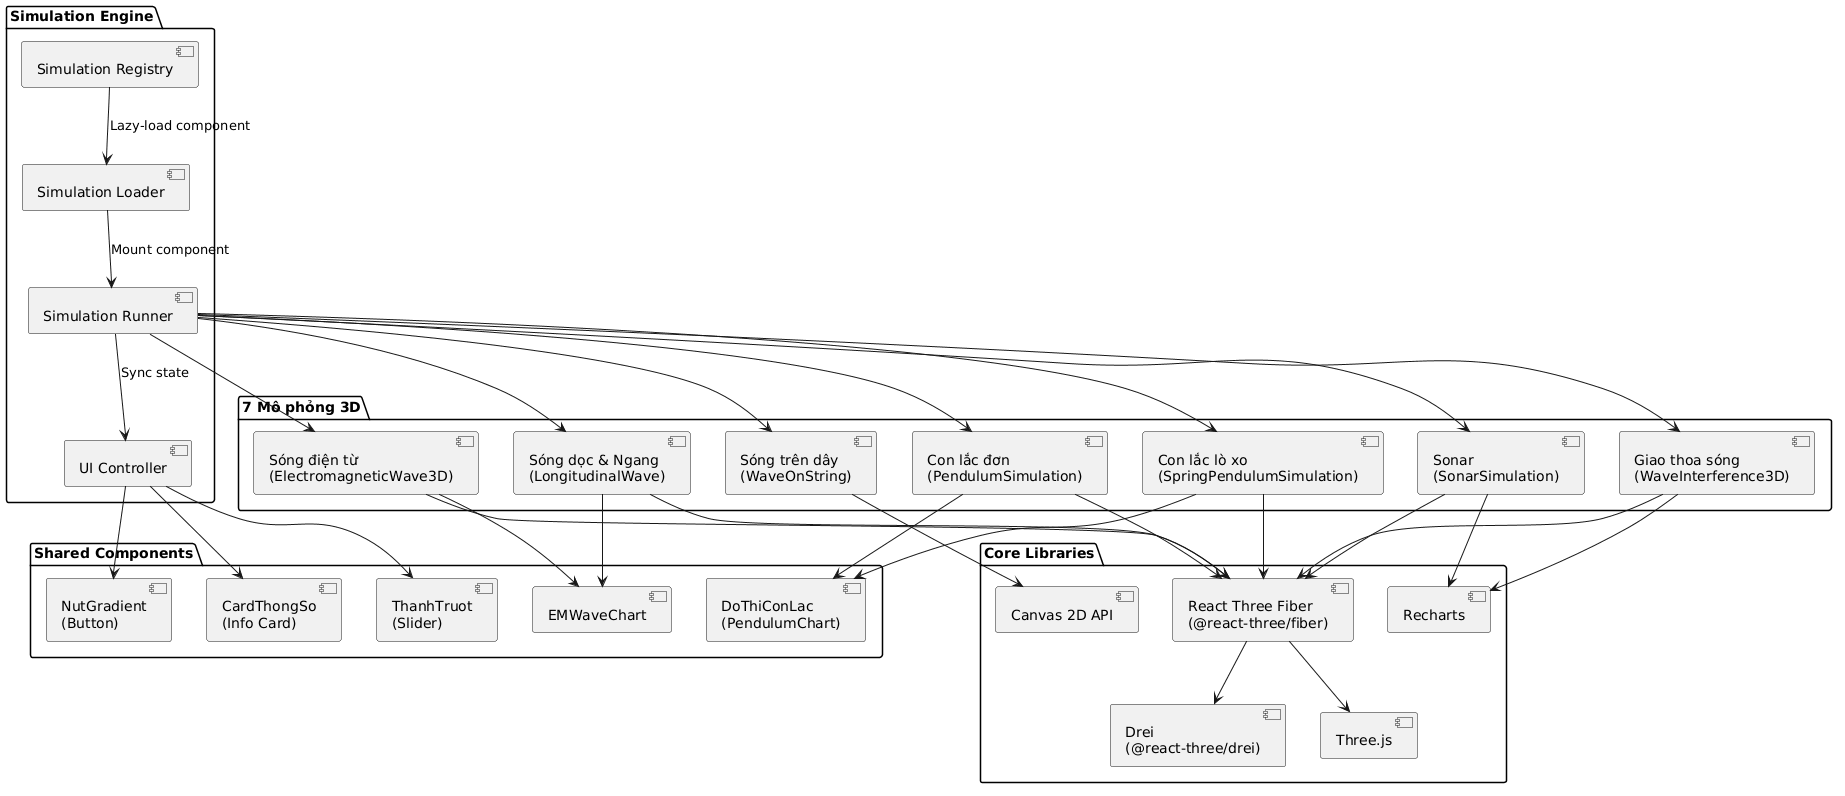
\includegraphics[width=0.9\textwidth]{Images/Phan_tich_Thiet_ke_he_thon/kiến_trúc_mô_phỏng.png}
    \vspace{0.5cm}
    \caption{Kiến trúc Simulation Engine – Plugin-Based}
    \label{fig:sim-arch}
\end{figure}


\subsection{Kiến trúc Component cho Một Mô phỏng Điển hình}

Mỗi mô phỏng 3D tuân theo một cấu trúc component nhất quán:

\begin{figure}[H]
\centering
\resizebox{\textwidth}{!}{
\begin{tikzpicture}[
    node distance=1.8cm,
    every node/.style={font=\small},
    box/.style={rectangle, rounded corners, draw, align=center},
    mainbox/.style={box, fill=blue!15, minimum width=11cm, minimum height=1.2cm},
    statebox/.style={box, fill=yellow!20, minimum width=11cm, minimum height=1cm},
    subbox/.style={box, minimum width=5cm, minimum height=2.2cm},
    vizbox/.style={subbox, fill=green!15},
    chartbox/.style={subbox, fill=orange!20},
    uibox/.style={box, fill=purple!15, minimum width=11cm, minimum height=1.2cm},
    arrow/.style={->, thick}
]

% Main
\node (main) [mainbox] 
{Component Chính\\\textbf{(ElectromagneticWaveSimulation)}};

% State
\node (state) [statebox, below of=main] 
{\textbf{State Management}\\
useState • useEffect • useMemo • useCallback};

% Visualization & Chart
\node (viz) [vizbox, below left=1.5cm and 0.5cm of state] 
{\textbf{3D Visualization}\\(EMWaveVisualization)};

\node (chart) [chartbox, below right=1.5cm and 0.5cm of state] 
{\textbf{Chart Component}\\(EMWaveChart)};

% UI
\node (ui) [uibox, below=3.5cm of state] 
{\textbf{UI Components}\\ThanhTruot • NutGradient • CardThongSo};

% Arrows
\draw[arrow] (main) -- (state);
\draw[arrow] (state) -- (viz);
\draw[arrow] (state) -- (chart);
\draw[arrow] (state) -- (ui);

\draw[arrow, dashed] (ui) -- node[right]{onChange} (state);

\end{tikzpicture}
}
\vspace{0.5cm}
\caption{Kiến trúc component của một mô phỏng điển hình}
\label{fig:component-arch}
\end{figure}
\textbf{Luồng dữ liệu trong một mô phỏng:}

\begin{enumerate}
    \item \textbf{UI Controls} (thanh trượt, checkbox, nút bấm) → gọi \texttt{setState} → cập nhật state trong Component Chính.
    \item State thay đổi → React re-render → props mới được truyền xuống 3D Visualization và Chart.
    \item \textbf{3D Visualization} sử dụng \texttt{useMemo} để tính toán lại hình học (tọa độ điểm sóng, vị trí vật...) dựa trên props mới.
    \item \textbf{Animation loop} (requestAnimationFrame hoặc useFrame) liên tục cập nhật \texttt{time} state → mỗi frame, 3D scene được render lại với vị trí/cường độ mới.
    \item \textbf{Dữ liệu lịch sử} (mảng góc, vận tốc, năng lượng...) được thu thập định kỳ → truyền xuống Chart Component → Recharts render biểu đồ.
\end{enumerate}


\section{Thiết kế Giao diện Người dùng (UI/UX Design)}

\subsection{Kiến trúc Layout Tổng quát}

Giao diện người dùng được thiết kế theo mô hình responsive với Tailwind CSS, hỗ trợ dark mode và ba breakpoints chính:

\begin{itemize}
    \item \textbf{Desktop} ($\geq$1024px): Layout 3 cột – Sidebar trái (danh sách bài học) | Nội dung chính (slide + mô phỏng) | Panel phải (thông số, điều khiển).
    \item \textbf{Tablet} (768px–1023px): Layout 2 cột – Ẩn sidebar, hiển thị nội dung chính + panel điều khiển dạng accordion.
    \item \textbf{Mobile} (<768px): Layout 1 cột – Tất cả nội dung xếp dọc, canvas 3D thu nhỏ.
\end{itemize}

\subsection{Các Module Giao diện Chính}

\begin{enumerate}
    \item \textbf{Slide Presentation Module}: Hiển thị nội dung bài học dưới dạng slide, hỗ trợ:
    \begin{itemize}
        \item Điều hướng bằng chuột (nút Next/Prev) và bàn phím (phím mũi tên).
        \item Hiển thị công thức toán học/vật lý bằng MathJax/KaTeX.
        \item Hình ảnh minh họa, bảng biểu, hộp thoại thảo luận (discussion-box), bài tập thực hành (practice-box).
        \item Thanh tiến trình slide.
    \end{itemize}
    
    \item \textbf{Simulation Module}: Nhúng mô phỏng 3D vào slide cuối của bài học, bao gồm:
    \begin{itemize}
        \item Canvas 3D (React Three Fiber) chiếm phần lớn không gian.
        \item Panel điều khiển với các tab: Bảng điều khiển (thanh trượt), Hiển thị (checkbox), Thông tin Vật lý (cards), Đồ thị Phân tích (Recharts).
        \item Overlay thông số thời gian thực (góc lệnh, vận tốc, thời gian...).
        \item Nút điều khiển: Play/Pause, Reset, Khóa camera, Toàn màn hình.
    \end{itemize}
    
    \item \textbf{Assessment Module}: Giao diện làm bài tập với:
    \begin{itemize}
        \item Bộ đếm thời gian.
        \item Thanh tiến trình câu hỏi.
        \item Hỗ trợ phím tắt 1-4 cho trắc nghiệm.
        \item Màn hình kết quả với điểm số, đáp án đúng/sai.
    \end{itemize}
    
\end{enumerate}

\section{Kết luận Chương 6}

Chương này đã trình bày chi tiết thiết kế hệ thống dựa trên phân tích cơ sở dữ liệu thực tế và kiến trúc công nghệ đã lựa chọn. Các nội dung chính bao gồm:

\begin{itemize}
    \item \textbf{Mô hình dữ liệu}: Các mối quan hệ được thiết kế tối ưu cho truy vấn nhanh và linh hoạt. Dữ liệu bài học được nhúng (embedded) để giảm số lượng truy vấn, trong khi tiến độ học tập và bài tập được lưu trong collection riêng để dễ dàng cập nhật.
    
    \item \textbf{Kiến trúc hệ thống}: Mô hình Full-Stack với Next.js 14, kết hợp SSR cho nội dung tĩnh và CSR cho mô phỏng 3D.
    
    \item \textbf{Luồng xử lý}: Hai luồng chính được mô tả chi tiết qua biểu đồ tuần tự: (1) Xem bài học và tương tác với mô phỏng 3D.
    
    \item \textbf{Kiến trúc mô phỏng 3D}: Mô hình plugin-based cho phép mỗi mô phỏng là một module độc lập, sử dụng chung các component UI (ThanhTruot, NutGradient, CardThongSo) và thư viện đồ họa (React Three Fiber, Drei, Three.js, Recharts, Canvas 2D).
    
    \item \textbf{Thiết kế UI/UX}: Giao diện responsive với 3 breakpoints, dark mode, và các module chức năng rõ ràng (Slide, Simulation, Assessment).
\end{itemize}

Các thiết kế này tạo nền tảng vững chắc cho việc triển khai xây dựng hệ thống, sẽ được trình bày chi tiết trong Chương 7.